
{
    \begin{frame}[plain]
        \begin{tikzpicture}[remember picture,overlay]
            \node[at=(current page.north),anchor=north] (head){
                
\includegraphics[width=0.9\paperwidth]{../intro/ipv-spyware-paper-head}
            };
            \node[at={([yshift=5mm]current page.south)},anchor=south] {
                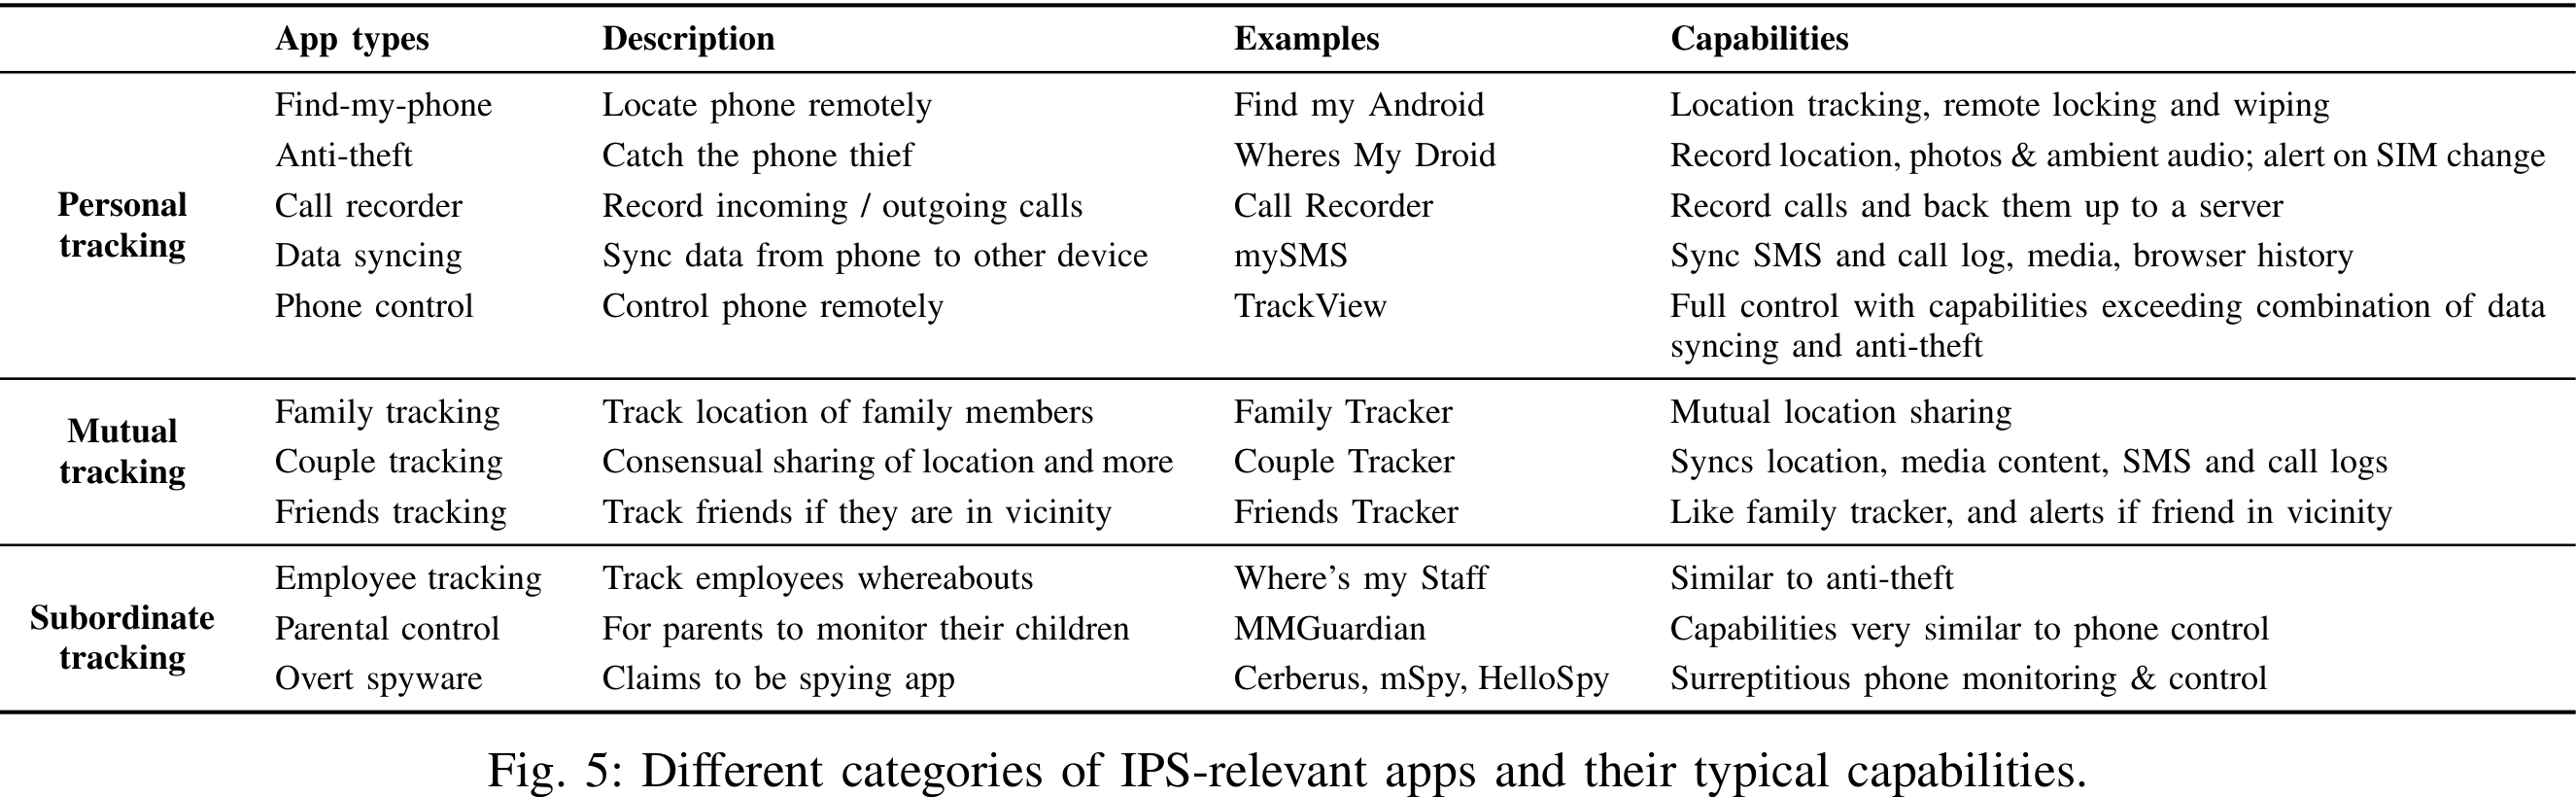
\includegraphics[width=0.98\paperwidth]{../intro/ipv-spyware-types}
            };
        \end{tikzpicture}
    \end{frame}
}

\begin{frame}{dual-use, context-sensitivity}
    \begin{itemize}
    \item this class: mostly talking about clearly anti-user software
        \begin{itemize}
        \item \ldots and how it tries to be covert
        \end{itemize}
    \vspace{.5cm}
    \item but there are also problems of \textit{dual-use} software
        \begin{itemize}
        \item phone tracking anti-theft software
        \item computer remote administration software
        \end{itemize}
    \item (also problems of intentionally `evil' software masquarding as legit)
        \begin{itemize}
        \item (e.g. marketted on ``how to spy on your \rule{1cm}{.5pt}'' blog)
        \item (e.g. unnecessairily well hidden when installed)
        \end{itemize}
    \item ideally, prevent ``bad'' use somehow
        \begin{itemize}
        \item phone OS should prevent \textit{covert} tracking?
        \item antimalware software should notice such software?
        \item \ldots
        \end{itemize}
    \end{itemize}
\end{frame}
